\section{Résultats}
\subsection{Résultats des évaluations de bcl2fastq et bcl-convert}
\subsubsection{Détermination des meilleurs paramètres pour bcl2fastq}
Après avoir effectué différentes combinaisons des paramètres, il a été mis en évidence que la variation du paramètre \texttt{r} et \texttt{w} en fixant le paramètre \texttt{p}, n'apportait pas de différences significatives pour le temps total d'exécution, le temps cpu ou le pourcentage d'utilisation cpu, comme on peut l'observer sur la figure \ref{barplot-param}, pour p fixé à 12. Des resultats similaires ont été obtenus pour p égale à 4, 8 et 16. 

\begin{figure}[H]
    \centering
    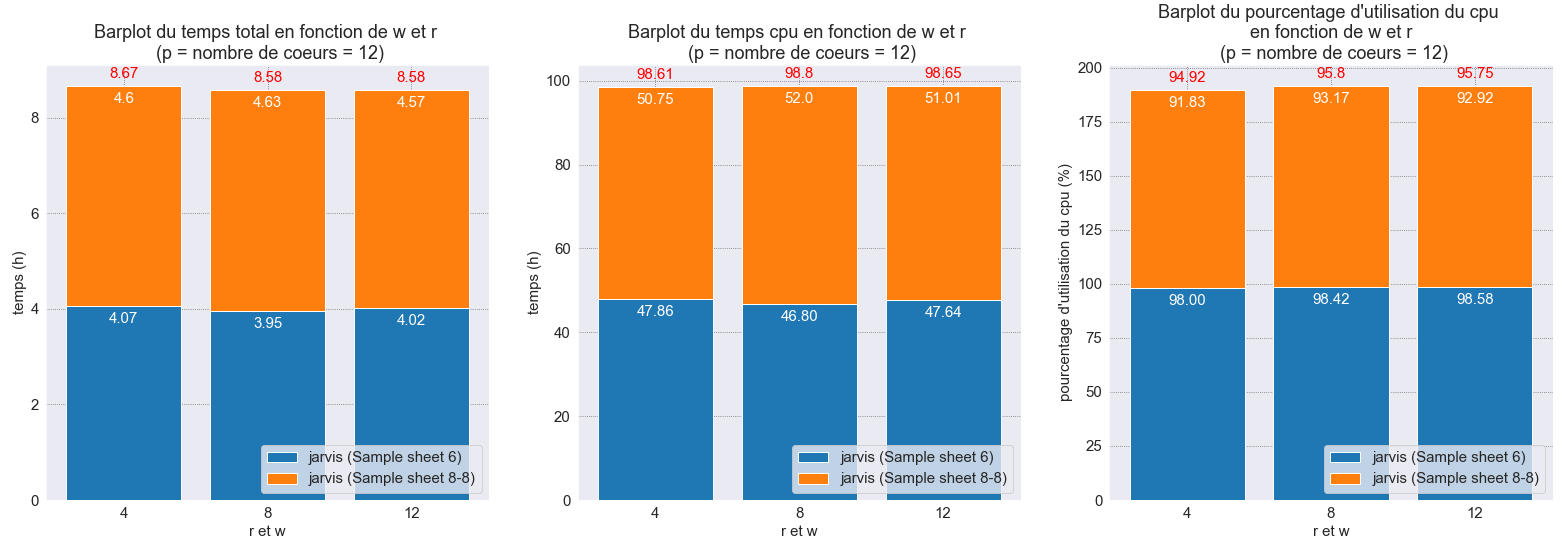
\includegraphics[width=0.8\textwidth]{img/barplot_cum_jarvis2.png}
    \caption{\footnotesize{Digrammes en bâtons du temps total d'éxécution (à gauche), temps cpu (au milieu) et du pourcentage d'utilisation des cpu (à droite) en fonction des paramètres r et w}}
    \label{barplot-param}
\end{figure}

Il y a deux \emph{sample sheet}\footnote{Fichier contenant les informations et instructions pour la génération des fastq et le démultiplexage}, car le nombre de bases considérées des \emph{reads index} entre les \emph{lanes} est différent, obligeant à réaliser deux appels différents au logiciel pour générer les fastq et le démultiplexage. Ci-dessous, la figure \ref{barplot-param2}, représente les résultats obtenus en faisant varier p et en fixant les paramètres r et w à 4 (ces deux paramètres sont fixés à 4 pour pouvoir comparer les 4 résultats). On observe que plus on augmente le nombre de cours et le nombre de \emph{threads} pour p, plus l'execution est rapide. On observe que le temps cpu augmente bien avec le nombre de cœurs et que le pourcentage d'utilisation des cpu est optimal (> 90\%).

\begin{figure}[H]
    \centering
    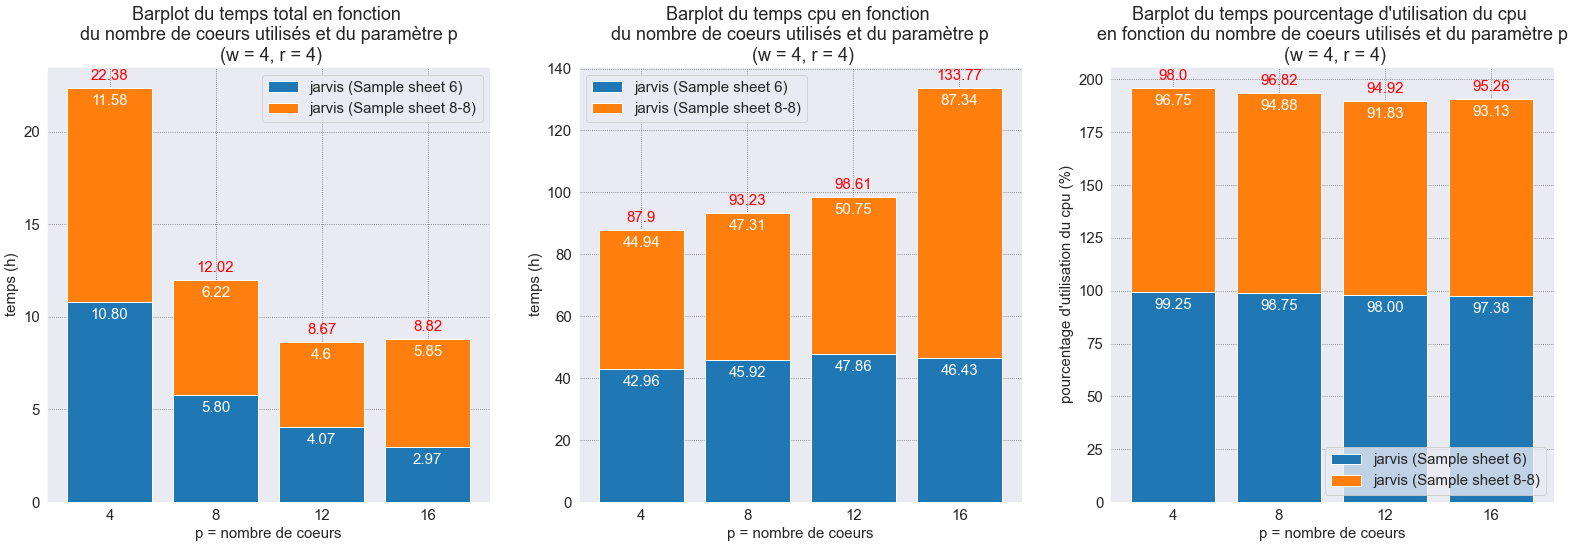
\includegraphics[width=0.8\textwidth]{img/barplot_cum_jarvis1.png}
    \caption{\footnotesize{Digrammes en bâtons du temps total d'éxécution (à gauche), temps cpu (au milieu) et du pourcentage d'utilisation des cpu (à droite) en fonction du paramètre p}}
    \label{barplot-param2}
\end{figure}

Au vue des résultats obtenus nous avons décidé que les meilleurs paramètres étaient de fixer p à 12, puisque le gain apporté en augmentant à 16 est faible. Néanmoins nous le conserverons pour réaliser la comparaison avec bcl-convert, tout comme p fixé à 8, car il nous permettrait de réaliser deux générations de fastq et de démultiplexage en simultané sur un seul noeud de calcul.\\

\subsubsection{Comparaison entre bcl2fastq et bcl-convert}
J'ai donc fait varier les paramètres \texttt{p}, \texttt{r} et \texttt{w} de manière à ce que chacun des paramètre soient égale au nombre de cœurs accordés aux deux logiciels. On observe bien, sur la figure \ref{fig-total-time}, que plus on augmente le nombre de cœurs pour chacun des logiciels (et donc le nombre de \emph{threads} pour \texttt{p}, \texttt{r} et \texttt{w}) plus la génération des fastq et le démultiplexage est rapide. De plus on remarque que bcl-convert permet de réduire le temps d'environs 1/3 par rapport à bcl2fatq. 

\begin{figure}[H]
    \centering
    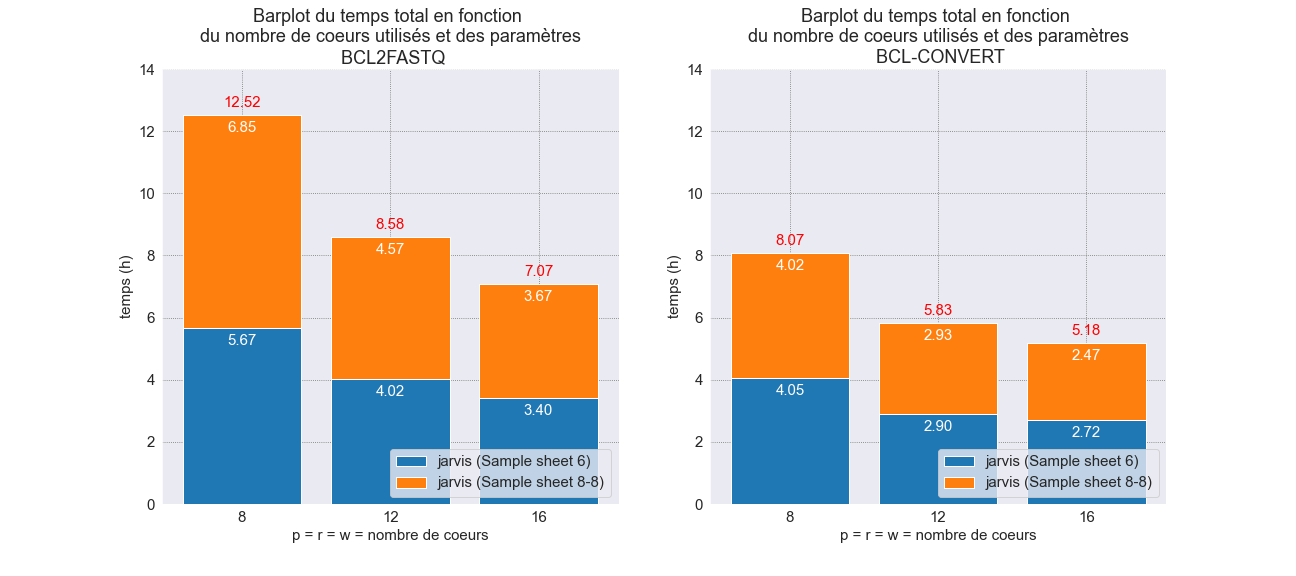
\includegraphics[width=1\textwidth]{img/barplot_total_time_comp.png}
    \caption{\footnotesize{Temps total de génération des fastq pour bcl2fastq et bcl-convert}}
    \label{fig-total-time}
\end{figure}

J'ai également échangé avec le service technique d'Illumina à propos des fichiers de sortie et de l'arborescence de bcl-convert. En effet il s'avère que l'arborescence et les fichiers de sortie sont très différents entre les deux logiciels. Ces échanges avaient pour objectif de savoir s'il on pouvait obtenir une arboresnce similaire à bcl2fastq, pour minimiser l'impact du changement de logiciel sur les pipelines. Le changement de bcl2fstq, qui sera bientôt obsolète, par bcl-convert va nous obliger à réaliser de gros changements dans tous les pipelines qui utilisent ces fichiers de sortie et va demander aussi au laboratoire de séquençage de s'adapter à la nouvelle \emph{sample sheet} de bcl-convert.

\subsubsection{Migration de bcl2fastq vers bcl-convert}
Le logiciel bcl-convert étant plus rapide d'environ 1/3 par rapport à bcl2fastq et que ce dernier sera bientôt obsolète. Sachant également, que le nombre de coeurs disponible par noeuds pour la partition \og \emph{production} \fg{}du cluster de calcul est de 16 coeurs. Nous avons décidé t'attribuer l'intégralité des coeurs d'un noeud de \og\emph{production} \fg{}, c'est à dire 16 coeurs. L'intégralité des changement entre les deux logiciels a été consignés dans un cahier des charges. Il contient, la commande à lancer pour réaliser le \emph{Base Calling}, les modules à charger dans l'environement, le chemin relatif des fichiers de sorties, ainsi qu'un exemple d'arborescence des fichiers de sorties. Ce qui permettera au développeur qui ce chargera de cette migration de suivre ce cahier des charges et ainsi faciliter la migration. Dû à la pression actuelle autour de la technologie MGI, c'est un autre développeur qui sera en charge de réaliser cette migration.

%==============================================================================%
%==============================================================================%

\subsection{Le pipeline de génération de fichiers de séquences pour la technologie MGI}
L'objectif du pipeline NGS\_RG\_MGI est de générer et distribuer les fichiers de séquences dans le bon répertoire de projet, d'échantillon, de type de séquençage et de run.
Tout en créant et mettant à jour les runs, pistes et readsets.
Notament concernant les métriques d'évaluations des ces derniers.
Le pipeline est composé de plusieurs grandes étapes.

\subsubsection*{Création et insertion des métriques du run et des pistes dans NGL }
La première étape consite à créer le run et ses pistes dans la base de données NGL, en y intégrant les métriques permettant d'évaluer le run et les pistes (figure \ref{NGL-screenshot_run-lane}).
Le nom du run est constitué de la date de séquençage, le nom du séquenceur et l'identifiant de la flowcell du run.\\

On y retrouve notament, le nombre total de reads (Nb Cluster (total)), le nombre de bases totales (Nb Bases (total)) générées par le run, la taille des reads et des index (Nb Cycles).
Concernant les pistes on retrouve le nombre total de bases et de reads générés sur la piste, le pourcentage de bases qui ont une qualité supérieur ou égale à Q30, Q20 et Q10. On a également le pourcentage de bases inconnus (\%N), ainsi que d'autres métriques qui permettent d'avaluer le run et les pistes. Celles-ci sont détaillées plus précisement en anexes (page \pageref{anexes1}).\\

\begin{figure}[H]
    \centering
    \fbox{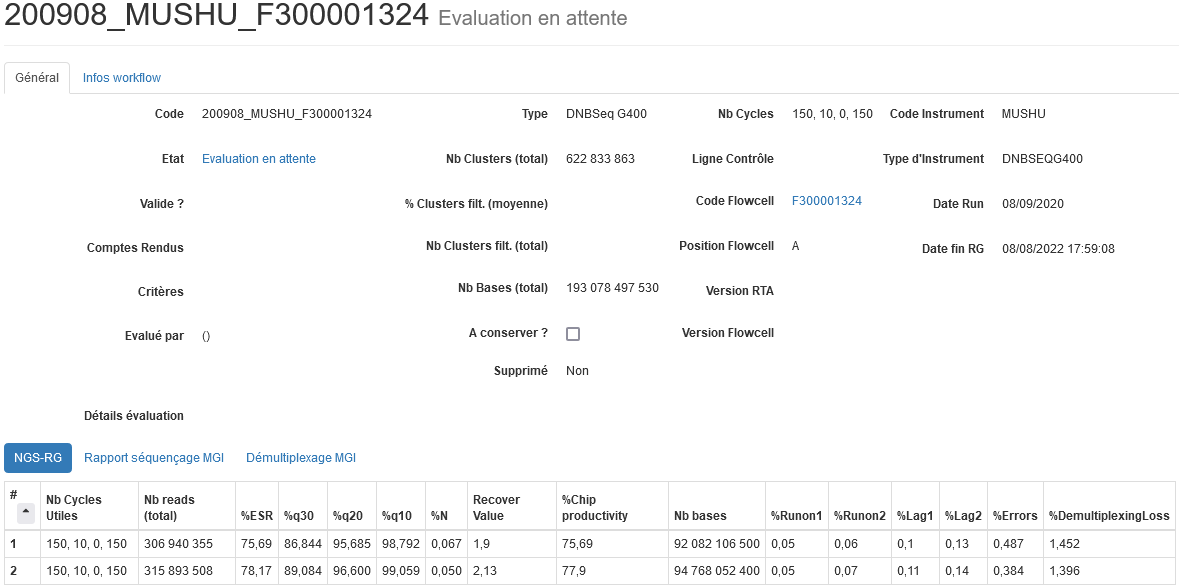
\includegraphics[width=1\textwidth]{img/NGL-screenshot_run-lane-ngsrg.png}}
    \caption{\footnotesize{Capture d'écran de la page du run 200908\_MUSHU\_F300001324 de NGL en cours de génération de fichiers de séquences (étapes d'ajout des métriques d'évaluation du run et des pistes).}}
    \label{NGL-screenshot_run-lane}
\end{figure}

\subsubsection*{Insertion des rapports de séquençage des pistes et de la listes des index dans NGL}
\begin{figure}[H]
    \centering
    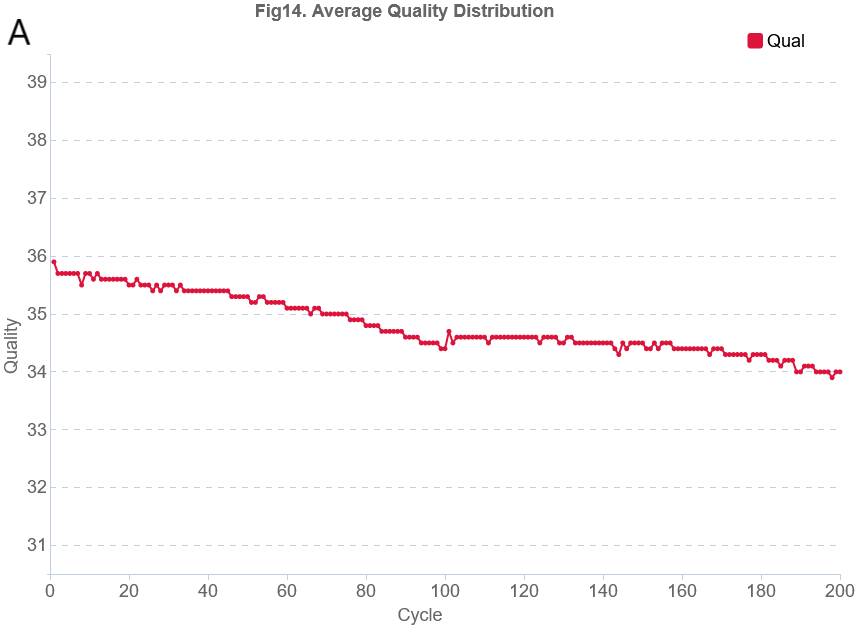
\includegraphics[width=0.45\textwidth]{img/mean_quality.png}
    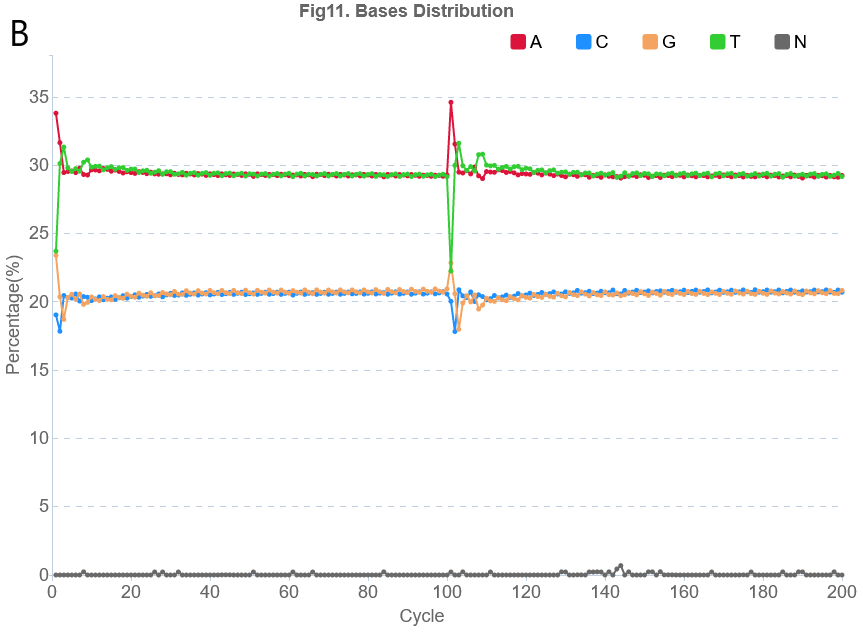
\includegraphics[width=0.45\textwidth]{img/bases_content.png}\\
    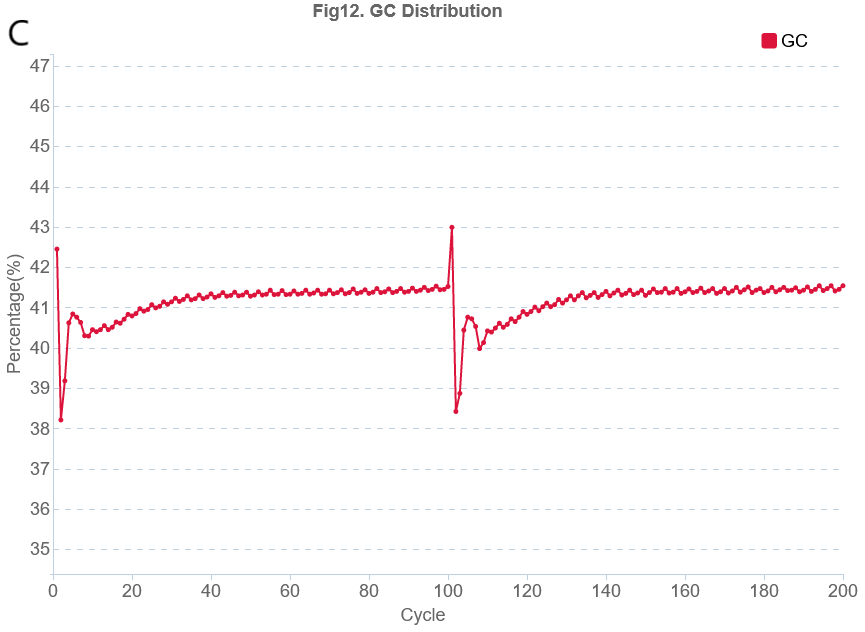
\includegraphics[width=0.45\textwidth]{img/GC_content.png}
    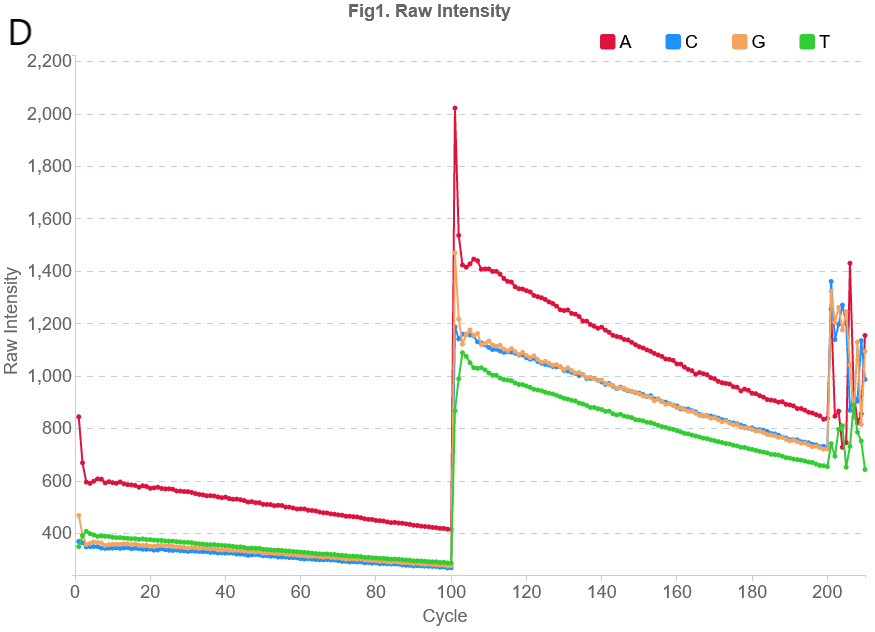
\includegraphics[width=0.45\textwidth]{img/raw_intensity.png}
    \caption{\footnotesize{Graphiques des distributions de la qualité moyenne (A), des bases nucléiques (B), du pourcentage de GC (C) et de l'intensité brut (D) au cours des cycles de séquençage}}
    \label{Graph-rapport-pistes}
\end{figure}

La seconde étape ajoute les rapports de séquençages des pistes que le séquenceurs génére en fin de séquençage.
Il s'agit de rapport html qui contiennent plusieurs tableaux de métriques et de graphiques permettant d'évaluer les pistes du run.
Il ya notament les graphiques de la distribution dela qualité moyenne en fonction des cycles (figure \ref{Graph-rapport-pistes}\textcolor{blue}{.A}), de la distribution des bases nucléiques en fonction des cycles (figure \ref{Graph-rapport-pistes}\textcolor{blue}{.B}), de la distribution du pourcentage de Guanine/Cytosine en fonction des cycles (figure \ref{Graph-rapport-pistes}\textcolor{blue}{.C}), de la distribution de l'intensité brut au cours des cycles (figure \ref{Graph-rapport-pistes}\textcolor{blue}{.D}).
Les tableaux et graphiques de ces rapports de séquençage permettent de facilité l'évaluation du run et de ses pistes.\\

Toujours dans l'optique de facilité l'évaluation du run et de ces pistes on ajoute, en troisième étape du pipeline, la liste des index représentée à plus de 0.01\% de la pistes, ainsi que les index attendus.
Ces index sont triés et affichés par ordre croissant dans NGL (figure \ref{top-index}).
Les index attendus sont colorés en vert et les index non-attendus ou inconnus sont colorés en rouge, ce qui permet de vérifier que les index attendus sont bien majoritairement représentés sur les pistes de la flowcell du run.

\begin{figure}[H]
    \centering
    \fbox{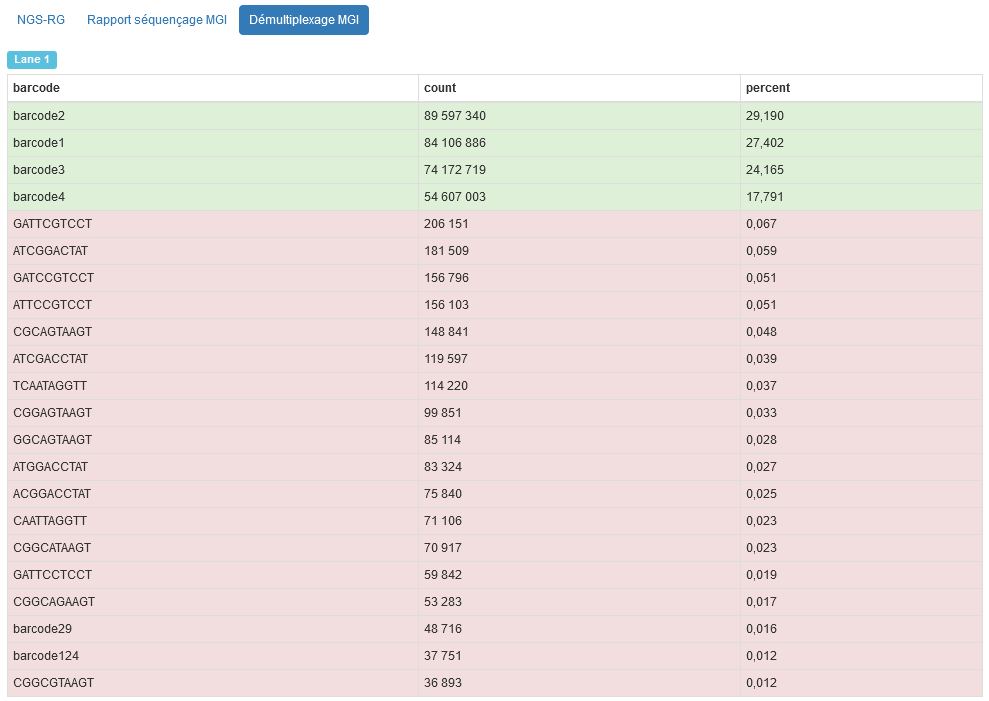
\includegraphics[width=1\textwidth]{img/Top_index.png}}
    \caption{\footnotesize{Capture d'écran de la page du run 200908\_MUSHU\_F300001324 de NGL en cours de génération de fichiers de séquences (onglet \og Démultiplexage MGI\fg{})}}
    \label{top-index}
\end{figure}

\subsubsection*{Concaténation des fichiers FASTQ d'un même readset}
Ensuite la quatrième étapes à pour objectif d'obtenir un seul fichier FASTQ par readset.
En effet la technologie MGI requiert une homogénéité de dépôt entre les différents index (aussi appelé\og barcode\fg{}) d'une piste.
Ce qui implique qu'il est possible d'avoir plusieurs index associés à un même index, donc qu'un échantillon peut être divisé en plusieurs fractions.
Le démultiplexage est directement réalisé par le séquenceur, il réalise le démultiplexage à partir des index connus (listes d'index fournis par MGI), on obtient donc un fichier FASTQ par index. Il est impossible de préciser au séquenceur quels index sont associés à un même readset pour le démulitiplexage.
Cette étape est donc essentielle pour obtenir un seul fichier FASTQ par readset.
Si le readset est associé à un seul readset alors on réalise une décompréssion du fichier FASTQ, si le readset est associé à plusieurs index alors on réalise une décompréssion et une concaténation des fichiers FASTQ, tout en le renommant dans un répertoire temporaire (cf. figure \ref{schema-concat-fastq}).

\begin{figure}[H]
    \centering
    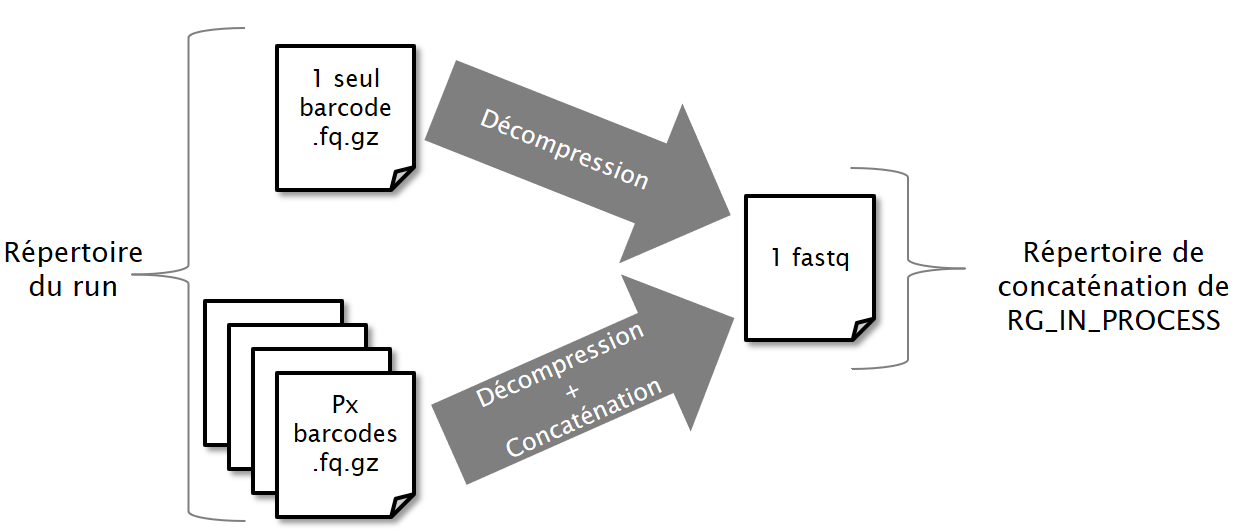
\includegraphics[width=0.8\textwidth]{img/Schéma_concaténation.png}
    \caption{\footnotesize{Schéma de l'étape de \og concaténation\fg{} des fichiers FASTQ d'un readset}}
    \label{schema-concat-fastq}
\end{figure}

\subsubsection*{Création et insertion des métriques des readset du run dans NGL}
La cinquiéme étape a pour objectif de permettre l'évaluation des readsets, en les créant et en insérant les métriques d'évaluation de ces derniers dans NGL (figure \ref{NGL-screenshot_readset}).
On y retrouve notamament le nombre de bases nucléiques et de reads du readset, ainsi que le pourcentage d'échantillon déposé sur la piste et le pourcentage de séquences valides par rapport au nombre total de séquences de la piste.
On y insère également certaines métriques du run dont le readset fait partie, comme le nombre de cycles des reads et des index, la date de run, ect. Toutes ces métriques sont décrites en annexes (page \pageref{anexes3})\\

Le nom du readset est condstitué de l'identifiant de projet, de l'identifiant du type de banque utilisée (ADN, ARN \dots), de l'identifiant d'échantillon, de l'indice de la lane, de l'identifiant de la flowcell et de l'identifiant du premier barcode.

\begin{figure}[H]
    \centering
    \fbox{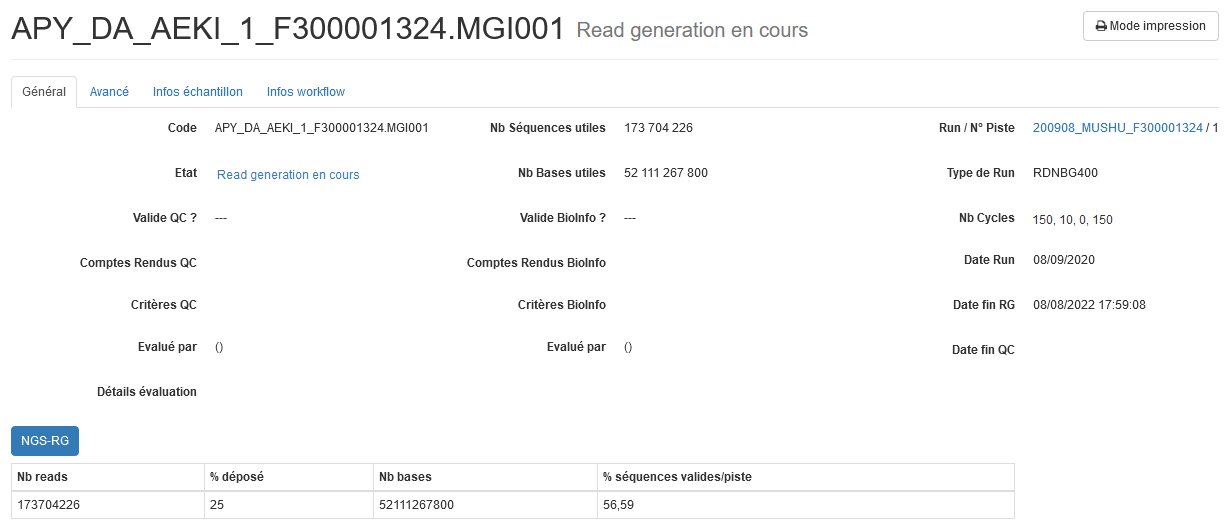
\includegraphics[width=1\textwidth]{img/NGL-screenshot_readset-ngsrg.png}}
    \caption{\footnotesize{Capture d'écran de la page du readset APY\_DA\_AEKI\_1\_F300001324.MGI001 de NGL en cours de génération de reads (étapes de création du readset et d'insertion de ces métriques d'évaluation)}}
    \label{NGL-screenshot_readset}
\end{figure}

On ajoute également la répartition des index au sein d'un readset (figure \ref{NGL-screenshot_readset-index}), ce qui permet de vérifier la composition en index du readset et de vérifier l'homogénéité de ces index au sein du readset.
Ce nom de readset est unique, ce qui permet de déterminer rapidement et simplement à quel projet, échantillon, ect appartiennent les fichiers séquences de ce readset.

\begin{figure}[H]
    \centering
    \fbox{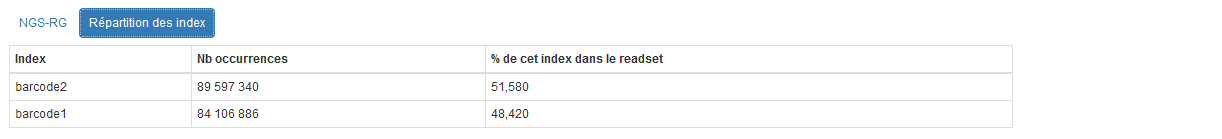
\includegraphics[width=1\textwidth]{img/NGL-screenshot_readset-index.png}}
    \caption{\footnotesize{Capture d'écran de la page du readset APY\_DA\_AEKI\_1\_F300001324.MGI001 de NGL en cours de génération de reads (onglet \og Répartition des index\fg{})}}
    \label{NGL-screenshot_readset-index}
\end{figure}

Au niveaux du run un tableau référençant les readsets et leurs métriques d'évaluation est également ajoutés (figure \ref{NGL-screenshot_tab-run-readset}).

\begin{figure}[H]
    \centering
    \fbox{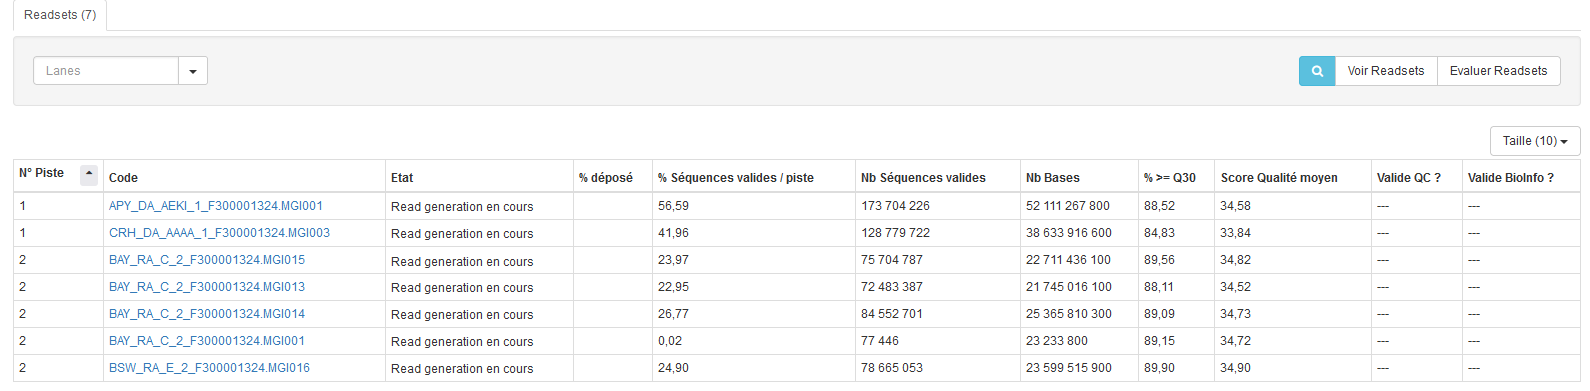
\includegraphics[width=1\textwidth]{img/NGL-screenshot_Tab-readset-in-run.png}}
    \caption{\footnotesize{Capture d'écran de la page du run 200908\_MUSHU\_F300001324 de NGL en cours de génération de fichiers de séquences (Tableau des readset du run)}}
    \label{NGL-screenshot_tab-run-readset}
\end{figure}

\subsubsection*{Renommage des fichiers séquences et insertion des méta-données dans NGL}
La sixième étape consiste à renomer les fichiers de séquences des readsets et d'insérer les méta-données de ces derniers dans NGL (figure \ref{meta-data-fastq}).
Le renommage des fichiers est nécessaire pour que chaque fichier de séquence ait un nom unique et \og parlant\fg{}.\\

\begin{minipage}{0.45\textwidth}
    \begin{figure}[H]
        \centering
        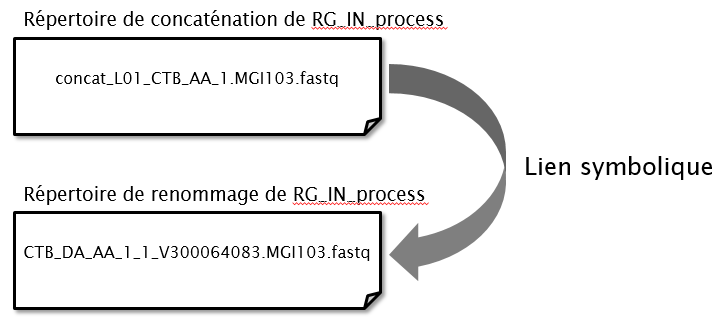
\includegraphics[width=1\textwidth]{img/Schema-renomage-fastq.png}
        \caption{\footnotesize{Schéma de l'étape de renommage des fichiers FASTQ d'un readset}}
        \label{schema-rename-fastq}
    \end{figure}
\end{minipage}
\hfill
\begin{minipage}{0.45\textwidth}
    Le nom doit permettre d'indentifier rapidement et simplement de quel projet, échantillon, flowcell, ect.
    appartient le fichier.
    Le renomage des fichiers est effectué en créant un lien symbolique des fichiers obtenus à l'étape de \og concaténation\fg{} dans un répertoire temporaire (cf figure \ref{schema-rename-fastq}).
\end{minipage}\\\\

Les méta-données, des fichiers de séquences du readset, qui sont insérées dans NGL permet aux utilisateurs de trouver rapidement l'emplacement de ces derniers sur le système de fichier, le type de fichier disponible (brut, nettoyer) et s'ils sont utilisable.
On y retrouve donc le chemin vers le repertoire de ces fichiers, leurs noms, leurs types, s'ils sont utilisable, s'il s'agit du read \emph{forward} ou \emph{reverse}, et le type d'encodage de la quality (Pour les séquenceurs MGI l'encodage est en ASCII 33).

\begin{figure}[H]
    \centering
    \fbox{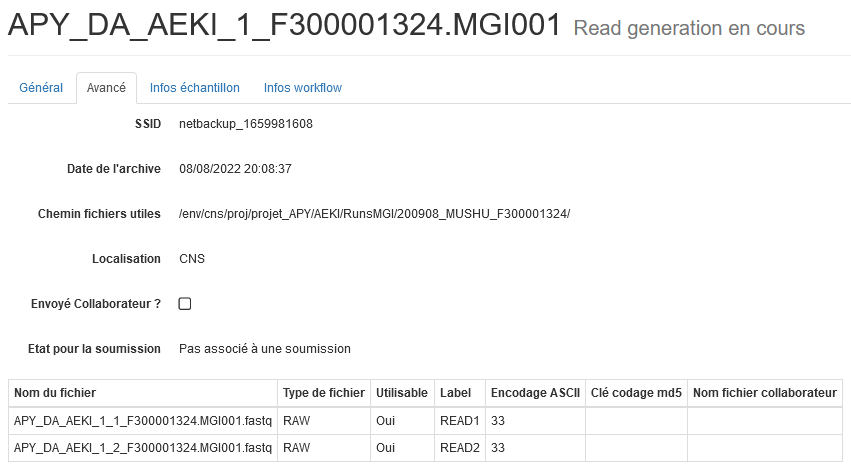
\includegraphics[width=1\textwidth]{img/meta-data-fastq.png}}
    \caption{\footnotesize{Capture d'écran de la page du readset APY\_DA\_AEKI\_1\_F300001324.MGI001 de NGL en cours de génération de fichiers de séquences (Onglet \og Avancé\fg{})}}
    \label{meta-data-fastq}
\end{figure}

\subsubsection*{Distribution des Fichiers séquences et des fichiers de statistiques}
La septième étape est de distribuer des fichiers de séquences \og attendus\fg{}, les fichiers de statistiques du run et les fichiers de séquences \og non attandus\fg{} dans leurs répertoires dédiés.
Les fichiers attendus sont copiés vers leurs répertoires finales si le séquençage a été effectué au genoscope.
Si ce dernier a été effectué au CNRGH, alors les fichiers sont copié et compressés.
Il y a cette différence entre les 2 centres, car le pipline de contrôle qualité prend en charge de fichiers compressés pour le CNRGH, contrairement à celui utilisé pour le Genoscope.\\

Les fichiers de statistiques du run sont archivés par pistes et par types (.html, .fq.stat) avant d'être copié vers leurs répertoires finales.
Ces fichiers sont conservés dans le cas où une métrique désirés ne fait pas partie de celles insérées dans NGL ou pour tout autres probléme qui nécéssiterait de récupérer les fichiers de statistiques du run.\\

Concernant les fichiers \og non attendus \fg{}, il s'agit des fichiers de séquence des index ne faisant pas partie d'un readset. Puisque lors du demultiplexage par les séquenceurs, on obtient un fichier FASTQ par index.
Ces fichier sont renomés et archivés, avant d'être distribués vers leur répertoire dédiés.
Ces fichers de séquences sont conservés dans l'éventualité d'une mauvaise déclaration d'index par les équpies de séquençage, pour pouvoir récupérer les fichiers fastq appartenant à cet index ou si l'on souhaite étudier les séquences des fichiers \og non-attendus\fg{}.\\

\subsubsection*{Mise à jour de fin de génération de fichiers de séquence dans NGL}
L'étape finale du pipeline de génération de fichiers de séquences pour la technologie MGI, est de mettre à jour le run et les readset dans l'état de \og fin de génération de reads\fg{}.
Cela entraine une mise à jour automatique du run à l'état \og d'évaluation en attente\fg{}, ce qui permet d'indiquer aux utilisateurs que le run peut être évalué.
Les readset sont aussi automatiquement mis à jour vers l'état \og d'attente de contrôle qualité\fg{}, permettant d'indiquer au pipeline de contrôle qualité qu'il peut effectuer le contrôle qualité des readset de ce run.

